\documentclass[10pt]{article}

\linespread{1} 
\usepackage{float}

\usepackage{geometry}
 \geometry{
  papersize={175mm,248mm},
 total={175mm,248mm},
 left=26mm,
 right=13mm,
 bottom=17mm,
 top=13mm,
 }

 


\usepackage{amsfonts,amssymb,graphicx,color}
\usepackage[font=small,labelfont=bf]{caption}
\usepackage{subcaption}

\usepackage{color, colortbl, framed}
\usepackage[T1]{fontenc}
\usepackage{mathptmx}

\usepackage{amsmath}
%\usepackage{lineno,hyperref}
\usepackage{authblk}
\usepackage{titlesec}

%\usepackage{epstopdf}

\usepackage{hhline}
\usepackage{xcolor,colortbl}
\renewcommand{\figurename}{Fig.}

%  \setcounter{secnumdepth}{0}
\usepackage{titlesec}
\titlespacing{\section}{0pt}{\parskip}{-\parskip}
\titlespacing{\subsection}{0pt}{\parskip}{-\parskip}
 \titleformat*{\section}{\normalfont\fontfamily{ptm}\fontsize{10}{19}\bfseries}
 \titleformat*{\subsection}{\normalfont\fontfamily{ptm}\fontsize{10}{18}\bfseries}

%\setlength{\columnsep}{6,3mm}


 \newcommand{\sgn}{\operatorname{sgn}}
\renewcommand{\abstractname}{}    % clear the title

\title{Segmentation algorithm of roadheader vibration signal based on the stable distribution parameters}
% \author{}
\author[1]{Jacek Wodecki}
\author[1]{Pawe{\l} Stefaniak}
\author[2]{Agnieszka Wy{\l}oma{\'n}ska}
\author[1]{Rados{\l}aw Zimroz}
\author[3]{Grzegorz {\.Z}ak}

\affil[1]{KGHM Cuprum Ltd, Research and Development Centre, Sikorskiego 2-8, 53-659 Wroclaw, Poland and Diagnostics and Vibro-Acoustic Science Laboratory, Wroclaw University of Technology, Wroclaw, Poland}

\affil[2]{Hugo Steinhaus Center, Department of Mathematics, Wroclaw University of Technology, Wroclaw, Poland}

\affil[3]{Diagnostics and Vibro-Acoustic Science Laboratory, Wroclaw University of Technology, Wroclaw, Poland}


\date{} 
\bibliographystyle{unsrtnat} 
\usepackage[square,numbers,sort&compress]{natbib}

% \biboptions{sort&compress}
\begin{document}

\maketitle
\textbf{Abstract.} In the real signal analysis the main problem is the non-stationarity of given data. The non-stationarity can be manifested in different ways. One of the possibility is the assumption that the signal is a mixture of different processes that exhibit different statistical properties. Thus before the further analysis the observed data should be segmented. In this paper we propose an automatic segmentation method which is based on $\alpha$-stable distribution approach. In the proposed procedure we estimate the parameters of stable distribution for consecutive sub-signals of given length and then by using expectation-maximization algorithm we classify the parameters. The obtained classes correspond to different segments of the signal. The proposed procedure we apply to the real vibration signal from roadheader working in mining industry. As a final result we obtained segments of real signal which constitute samples of different behaviors and are related to different modes of operation of the machine. \newline \newline
\textbf{Keywords:} segmentation, stable distribution, expectation-maximization algorithm, roadheader.

\section{Introduction}

Analysis and modeling of real signals measured by advanced data acquisition systems provide possibility to obtain information about the considered process. Very often observed time series exhibits strong non-stationary behavior resulting from the fact that it consists of not one but multiple processes that coexist or occur one after the other.  In most of the cases those processes cannot be analyzed by the same tools because they exhibit completely different character and have different statistical properties. Sometimes the processes can be described by the same or similar models but their parameters differ. Therefore before the modeling of given signal its preliminary segmentation should be performed.
One of the most fundamental reason for segmentation is extraction of parts (segments) of the signal with homogenous properties. Segmentation is also related to finding such time points where the signal changes the properties and switches to the other regime \cite{lopatka2005non,wylomanska2015identification,gajda44regime,wylomanska2014signal}. 
There are many segmentation methods and during recent years number of papers in this field  has increased. Segmentation techniques are very often dedicated to applications for which they were used. Some of the methods are based on special behavior of the signal in time domain \cite{lopatka2005non,gajda44regime,makowski2013procedure} however there are also methods which are based not on the raw signal but on its transformations to other domains \cite{obuchowski2014local}.
Signal segmentation has been applied in many areas. It is especially crucial in condition monitoring (to isolate shocks related to damage) \cite{obuchowski2014local}, machine performance analysis (to find when machine operates under overloading, idle mode etc.) \cite{wylomanska2014signal}, experimental physics \cite{gajda44regime}, biomedical signals (like ECG signals) \cite{azami2012improved}, speech analysis \cite{makowski2014automatic} and in seismic signal analysis \cite{popescu2014signal}.In this paper we are especially interested in the first two mentioned applications.
In this paper we propose the segmentation method which is based on the modeling of given signal by $\alpha$-stable distribution and on the expectation-maximization algorithm. The stable distributions are especially important in the context of modeling of data with visible peaks but it should be mentioned that for $\alpha$ parameter equal to 2 the stable distribution reduces to Gaussian one. There are many applications of such distributions like finance, environmental engineering or condition monitoring \cite{zak2014application}. The expectation-maximization algorithm was invented for finding maximum likelihood or maximum a posteriori estimates of parameters in statistical models, where the model depends on unobserved latent variables. However this algorithm very often is applied in the classification problem. In the proposed technique for the application to raw two-channel signal first we estimate the appropriate parameters of stable distribution and then by using expectation-maximization algorithm and Silhouette criterion we classify the data. We apply this procedure to the real vibration signal from roadheader working in the mining industry. Investigated machine is one of the most crucial components of the technological process in underground mining industry. It eliminates blasting operations in exploitation area and ensures continuous mechanical drilling. There exist many factors having influence on vibration signal profile (various physical and mechanical properties of deposit, design features of the machine, depth of drilling, motion parameters and wear level of machine elements). Appropriate segmentation of vibration signal allows for identification of spectrum domain components corresponding to different processes.

\section{Methodology}
The segmentation procedure of roadheader vibration signal is based on the alpha-stable distribution approach. As it was mentioned, the $\alpha$-stable distribution is an extension of Gaussian one, namely for some values of parameters ($\alpha$=2) it reduces to normal distribution. A random variable X is an $\alpha$-stable distributed if its characteristic function takes the following form:

\begin{equation}
Ee^{itX} =
  \begin{cases}
    e^{\left(-\Sigma^\alpha |t|^\alpha \left(1-\beta \sgn(t)\tan\left(\frac{\pi\alpha}{2}\right) \right) +i\mu t \right)},    & \quad \alpha \neq 1\\
    e^{\left(-\Sigma |t| \left(1+i\beta sgn(t)\frac{2}{\pi}\right) +i\mu t \right)},  & \quad \alpha = 1
  \end{cases}
  \label{eq1}
\end{equation}

where $\alpha$ (0 < $\alpha$ $\leq$ 2) is stability parameter, $\beta$ (-1 $\leq$ $\beta$ $\leq$ 1)is asymmetry parameter, $\Sigma$($\Sigma$ > 0)  is scale parameter and $\mu$ ($\mu$ $\in$ R) is location parameter. Of the four parameters defining the family of stable distribution, most attention has been focused on the stability parameter, $\alpha$. The $\alpha$-stable distributed random variable has 'heavy' tails, i.e. its cumulative probability density function decays with power law. Therefore, there is a high probability of the variable having extreme values, which is useful in modelling of impulsive signal \cite{zak2014application}. The other distribution that can be useful in impulsive signal modelling is presented in \cite{stefaniak2015procedures}.
In our segmentation procedure first the raw signal is divided into consecutive sub-signals of length N samples. The sub-signals overlap by K$\%$. Next, for each sub-signal the empirical standard deviation ($\sigma$) is calculated. Because the sub-signals exhibit behavior related to heavy tailed data (visible jumps), then we propose to model the data by stable distribution and the next parameters taken to the classification are $\alpha$ and $\Sigma$. In the literature one can find different estimation methods that can be used here \cite{allen1977short,samorodnitsky1994stable}. In this paper we apply the regression method which is based on the characteristic function of the considered distribution (see Eq.\ref{eq1}).
As a final step, the mentioned parameters ($\sigma$,$\alpha$,$\Sigma$) are used in the expectation-maximization algorithm to the classification. We normalize the data before the further analysis. We should mention that in the analysis we consider two-channel signal and for sub-signals for each of them we estimate the parameters therefore in the expectation-maximization algorithm we take under consideration six parameters. 
In statistics, an expectation-maximization (EM) algorithm is an iterative method for finding maximum likelihood or maximum a posteriori estimates of parameters in statistical models, where the model depends on unobserved latent variables. The EM iteration alternates between performing an expectation (E) step, which creates a function for the expectation of the log-likelihood evaluated using the current estimate for the parameters, and a maximization (M) step, which computes parameters maximizing the expected log-likelihood found on the E step. These parameter-estimates are then used to determine the distribution of the latent variables in the next E step \cite{dempster1977maximum,sundberg1974maximum,neal1998view,hastie2001algorithm}. EM is frequently used for data clustering in machine learning and computer vision. In natural language processing, two prominent instances of the algorithm are the Baum-Welch algorithm and the inside-outside algorithm for unsupervised induction of probabilistic context-free grammars. In our procedure we also propose to estimate number of clusters with Silhouette criterion \cite{kaufman2009finding,rousseeuw1987silhouettes} for limited range of number of clusters k (in our application k=1:5) with the measure of distance set to Euclidean.
In Fig. \ref{fig:block} we present the scheme of our segmentation procedure.

\begin{figure}[h!]
\centering
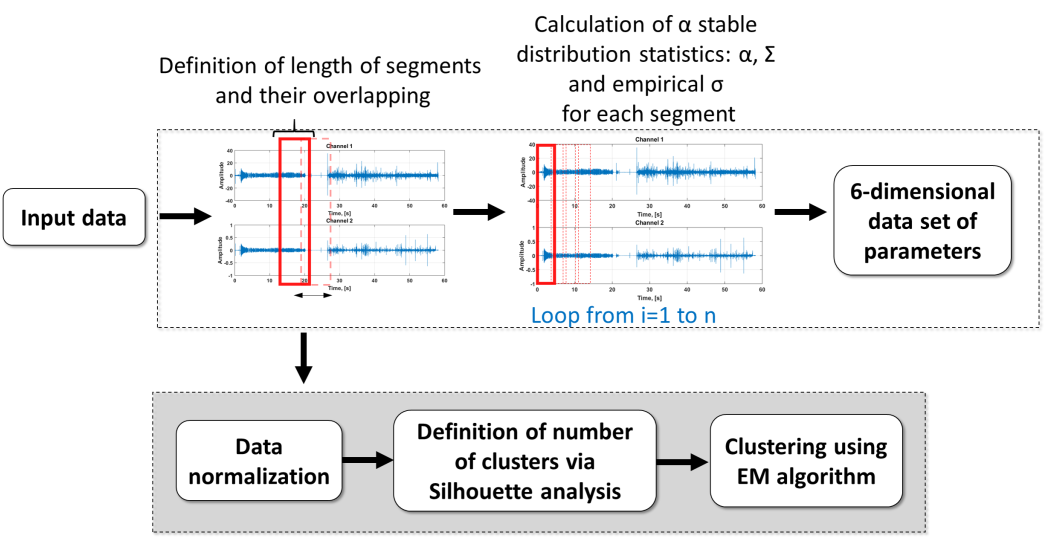
\includegraphics[width=0.8\textwidth]{wykresy/block}
\caption{Scheme of the segmentation procedure}
\label{fig:block}
\end{figure}

\section{Real signal analysis}

The analyzed real data set represents vibration signal of a roadheader. The sampling frequency $F_s$ = 25 kHz. Measurement was performed by using two accelerometers placed orthogonally on the mining head's arm. Duration of measurement was equal to 60 seconds. The analyzed two-channel data set is presented in Fig. \ref{fig:raw}. 

\begin{figure}[h!]
\centering
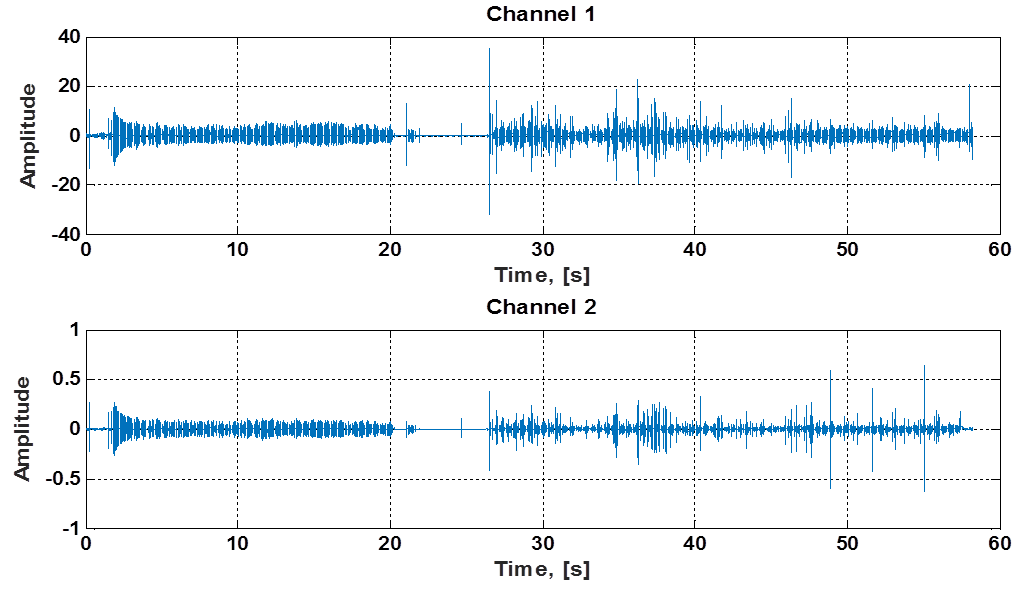
\includegraphics[width=0.6\textwidth]{wykresy/raw}
\caption{The two-channels raw roadheader vibration signal}
\label{fig:raw}
\end{figure}

According to the presented  segmentation procedure we divide the two-channel raw signal into sub-signals consisting of 10000 observations with overlap 50$\%$. Next, for each sub-signal the standard deviation and two parameters related to $\alpha$-stable distributions are calculated. In Fig. \ref{fig:stats} we present the estimated parameters for sub-signals corresponding to both analyzed channels.

\begin{figure}[h!]
\centering
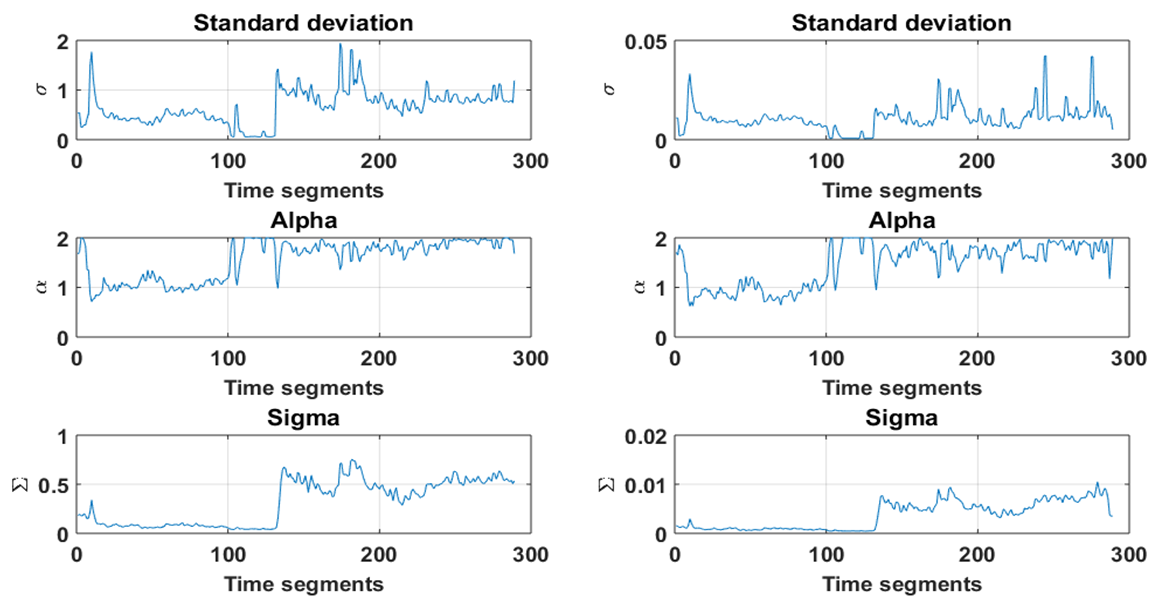
\includegraphics[width=0.9\textwidth]{wykresy/stats}
\caption{The estimated parameters ($\sigma$,$\alpha$,$\Sigma$) for sub-signals (segments) related to two-channels vibration signal}
\label{fig:stats}
\end{figure}

This set of six statistics represents set of N points $\chi$ in six-dimensional feature space, within which we perform clustering. Dataset $\chi$ is then centered and variance over each dimension is set to 1. This operation allows to more reliable and efficient cluster amount analysis.
After obtaining the set of parameters we estimate number of clusters with Silhouette criterion for limited range of number of clusters \textit{k=5}. When optimal number of clusters \textit{k} is estimated, EM algorithm performs clustering of the dataset $\chi$ splitting it into \textit{k} classes. For the analyzed signal we obtain that the optimal number of clusters is equal to four. In Fig. \ref{fig:out} we present the division of the raw signal from the first channel (left panels) and second channel (right panels) into four clusters.

\begin{figure}[!ht]
  \centering
  \begin{subfigure}[b]{0.49\textwidth}
      \centering
     % \captionsetup{skip=0.01pt}
      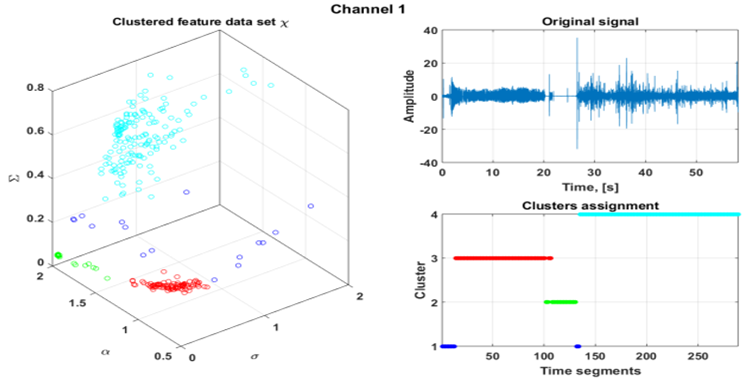
\includegraphics[width=\textwidth]{wykresy/out1}
      \caption{Channel 1}
      \label{fig:out1}
  \end{subfigure}
  %\hfill
  \begin{subfigure}[b]{0.49\textwidth}
      \centering
    %  \captionsetup{skip=0.01pt}
		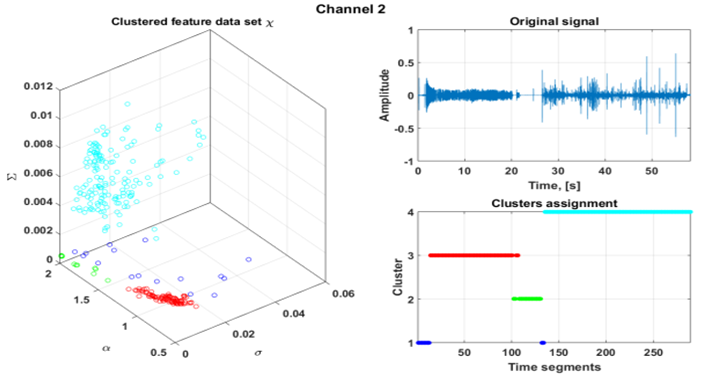
\includegraphics[width=\textwidth]{wykresy/out2}
        \caption{Channel 2}
    \label{fig:out2}
  \end{subfigure}
  \caption{Result of data clustering. Data points in part a) are displayed as features of signal corresponding to appropriate channel in 3-dimensional space for presentational purpose, however they were analyzed and clustered in 6 dimensions. Data is also presented in the form before centering and variance normalization for clear visual interpretation; b) analyzed raw signal; c) association of data points to clusters in the function of time for comparison with original signal above it.}
  \label{fig:out}
\end{figure}

As a result of the presented procedure we obtain segments belonging to certain clusters. We can apply the technique once again to data from one clustering in order to identify processes inside it, i.e.to make the so-called  "next-layer analysis". As an example, we consider part of the third cluster presented in red color in Fig. \ref{fig:out}. For this cluster we observe that there are regions of denser and more sparse impulses that  suggests the segment is a mixture of different processes with different statistical properties, see Fig. \ref{fig:raw2}. By using presented methodology we separate the data into classes. 

\begin{figure}[h!]
\centering
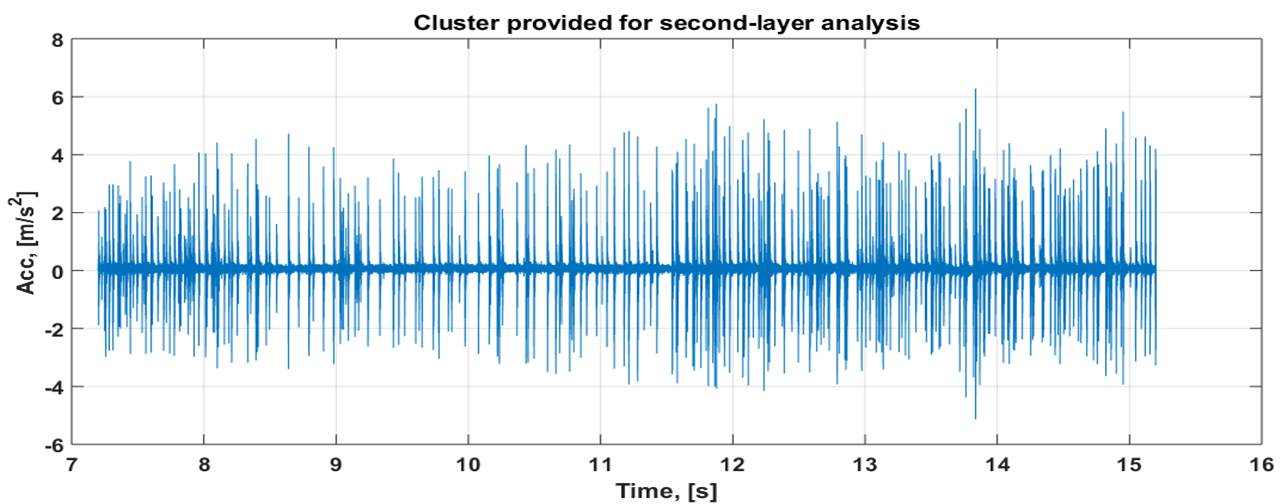
\includegraphics[width=0.9\textwidth]{wykresy/raw2}
\caption{Third cluster (marked in red in Fig. \ref{fig:out}) from channel 1}
\label{fig:raw2}
\end{figure}

For the signal related to the third cluster we apply the introduced technique. In this case the Silhouette evaluation estimated two clusters and results of EM clustering are presented in Fig. \ref{fig:outt}.

\begin{figure}[!ht]
  \centering
  \begin{subfigure}[b]{0.49\textwidth}
      \centering
     % \captionsetup{skip=0.01pt}
      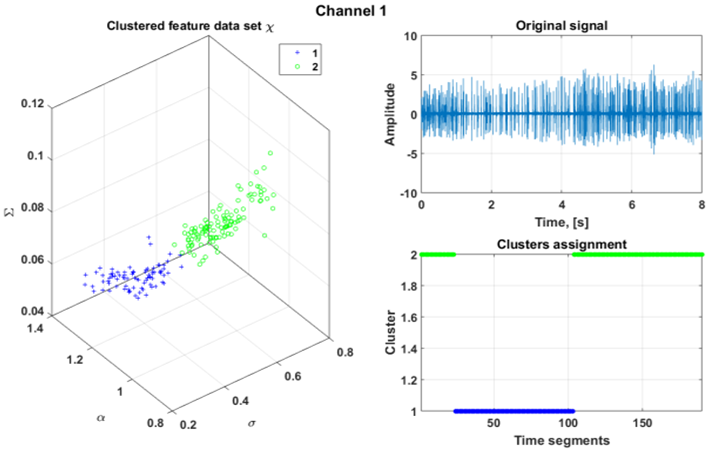
\includegraphics[width=\textwidth]{wykresy/out3}
      \caption{Channel 1}
      \label{fig:out3}
  \end{subfigure}
  %\hfill
  \begin{subfigure}[b]{0.49\textwidth}
      \centering
    %  \captionsetup{skip=0.01pt}
		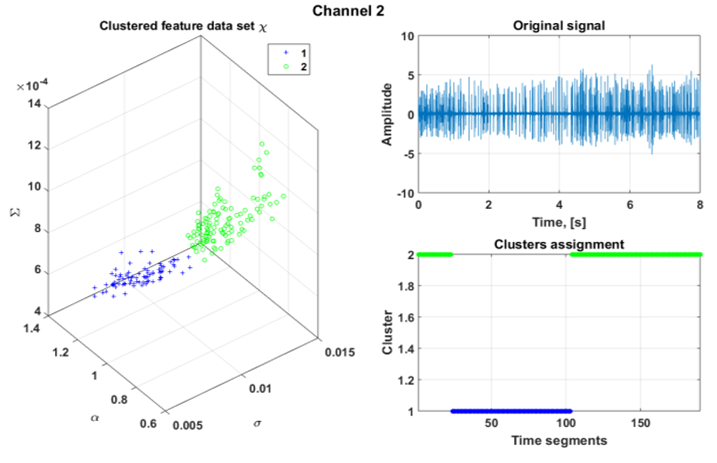
\includegraphics[width=\textwidth]{wykresy/out4}
        \caption{Channel 2}
    \label{fig:out4}
  \end{subfigure}
  \caption{Second-layer analysis of the third cluster. Distinction of two separate groups is clearly visible}
  \label{fig:outt}
\end{figure}

In practice we can proceed with as many layers as we wish, since number of layers can be provided as a parameter to the implemented algorithm. Although it is a good practice to limit search space of Silhouette estimation to about 2-3 clusters for deeper layers, and proceed with no more than 2-3 layers of analysis. If we go past those recommendations, results will make no sense since algorithm will greedily try to find clusters even as single points.

\section{Summary}

In this paper we have proposed  a new segmentation technique which can be applied to the vibration signal from roadheader working in the mining industry. Very harsh mining conditions, presence of many sources of interferences and many different operation modes have impact on the difficulty of signal analysis, for example in the diagnostic point of view. Therefore it is necessary to develop a novel technique for signal segmentation in order to identify different operational modes. The proposed methodology is automatic and  based on the stable distribution approach, Silhouette criterion and expectation-maximization algorithm applied in last step of the procedure, i.e. to the classification of the appropriate parameters. As a result we obtain the time periods for which the analyzed signal has homogenous structure. The obtained segments correspond to different  modes of operation of the machine. Furthermore, detection and parameterization of such events might help to improve efficiency of machine usage, for example to minimize number of segments and their duration for machine operation under idle mode or overload mode.

\section*{Acknowledgements}

This work is partially supported by the statutory grant No.S40128 and No.S50112 (G. Zak).

% \bibliographystyle{IJMRE_style}
\bibliography{mybibfile}


\end{document}